\documentclass{article}
\usepackage[utf8]{inputenc}
\usepackage[spanish]{babel}
\usepackage{graphicx}	%Si se quiere compilar con las imagenes
% \usepackage[draft]{graphicx}	%Si NO se quiere compilar con las imagenes porque tarda mucho
\usepackage{graphics, float, fancyhdr, titling, caption, subcaption}
\usepackage{listings}
\usepackage[a4paper, total={6in, 9.5in}]{geometry}
\usepackage{fancyhdr}
\usepackage{hyperref}		% solo se debe usar si se quiere usar \hypersetup
\usepackage{xurl}


% \usepackage{amsmath}      % Si se quiere usar \text{texto} dentro del modo matematico
%\setcounter{secnumdepth}{-2}       %Poner solo esto si no se quieren numero delante de las secciones y niveles inferiores.

\renewcommand{\footrulewidth}{0.4pt}
\title{

\includegraphics[width=1.75in]{imagenes/UGR-Logo.png} \\
\vspace*{1in}
\textbf{Cuestiones Tema X} \\
Animación por Ordenador \\
\vspace*{0.5in}}
\author{Andrés Merlo Trujillo \\
andresmerlo@correo.ugr.es \\
77147239H \\ 
\vspace*{0.5in} \\
E.T.S. de Ingenierías Informática y de Telecomunicación \\
\textbf{Universidad de Granada}} \date{\today}

\hypersetup{
    colorlinks=true,
    linkcolor=black,
    citecolor=black
}

\renewcommand\maketitlehooka{\null\mbox{}\vfill}
\renewcommand\maketitlehookd{\vfill\null}

\begin{document}
\begin{titlingpage}
\maketitle
\end{titlingpage}

\tableofcontents

\newpage

\pagestyle{fancy}   %a partir de comienza el header (se salta el indice y portada)
\fancyhead[L]{Andrés Merlo Trujillo}
\fancyhead[R]{Animación por Ordenador}
%\section{Ejercicio 1}
%\begin{figure}[H]
%    \centering
%    \includegraphics[width=\textwidth]{imagenes/passwdfile.png}
%    \vspace{10pt}
%    \footnotesize{Fuente: https://...}
%\end{figure}

% \begin{figure}[H]
%     \centering 
% 	\begin{subfigure}[t]{0.48\textwidth}
% 	    \centering
% 	    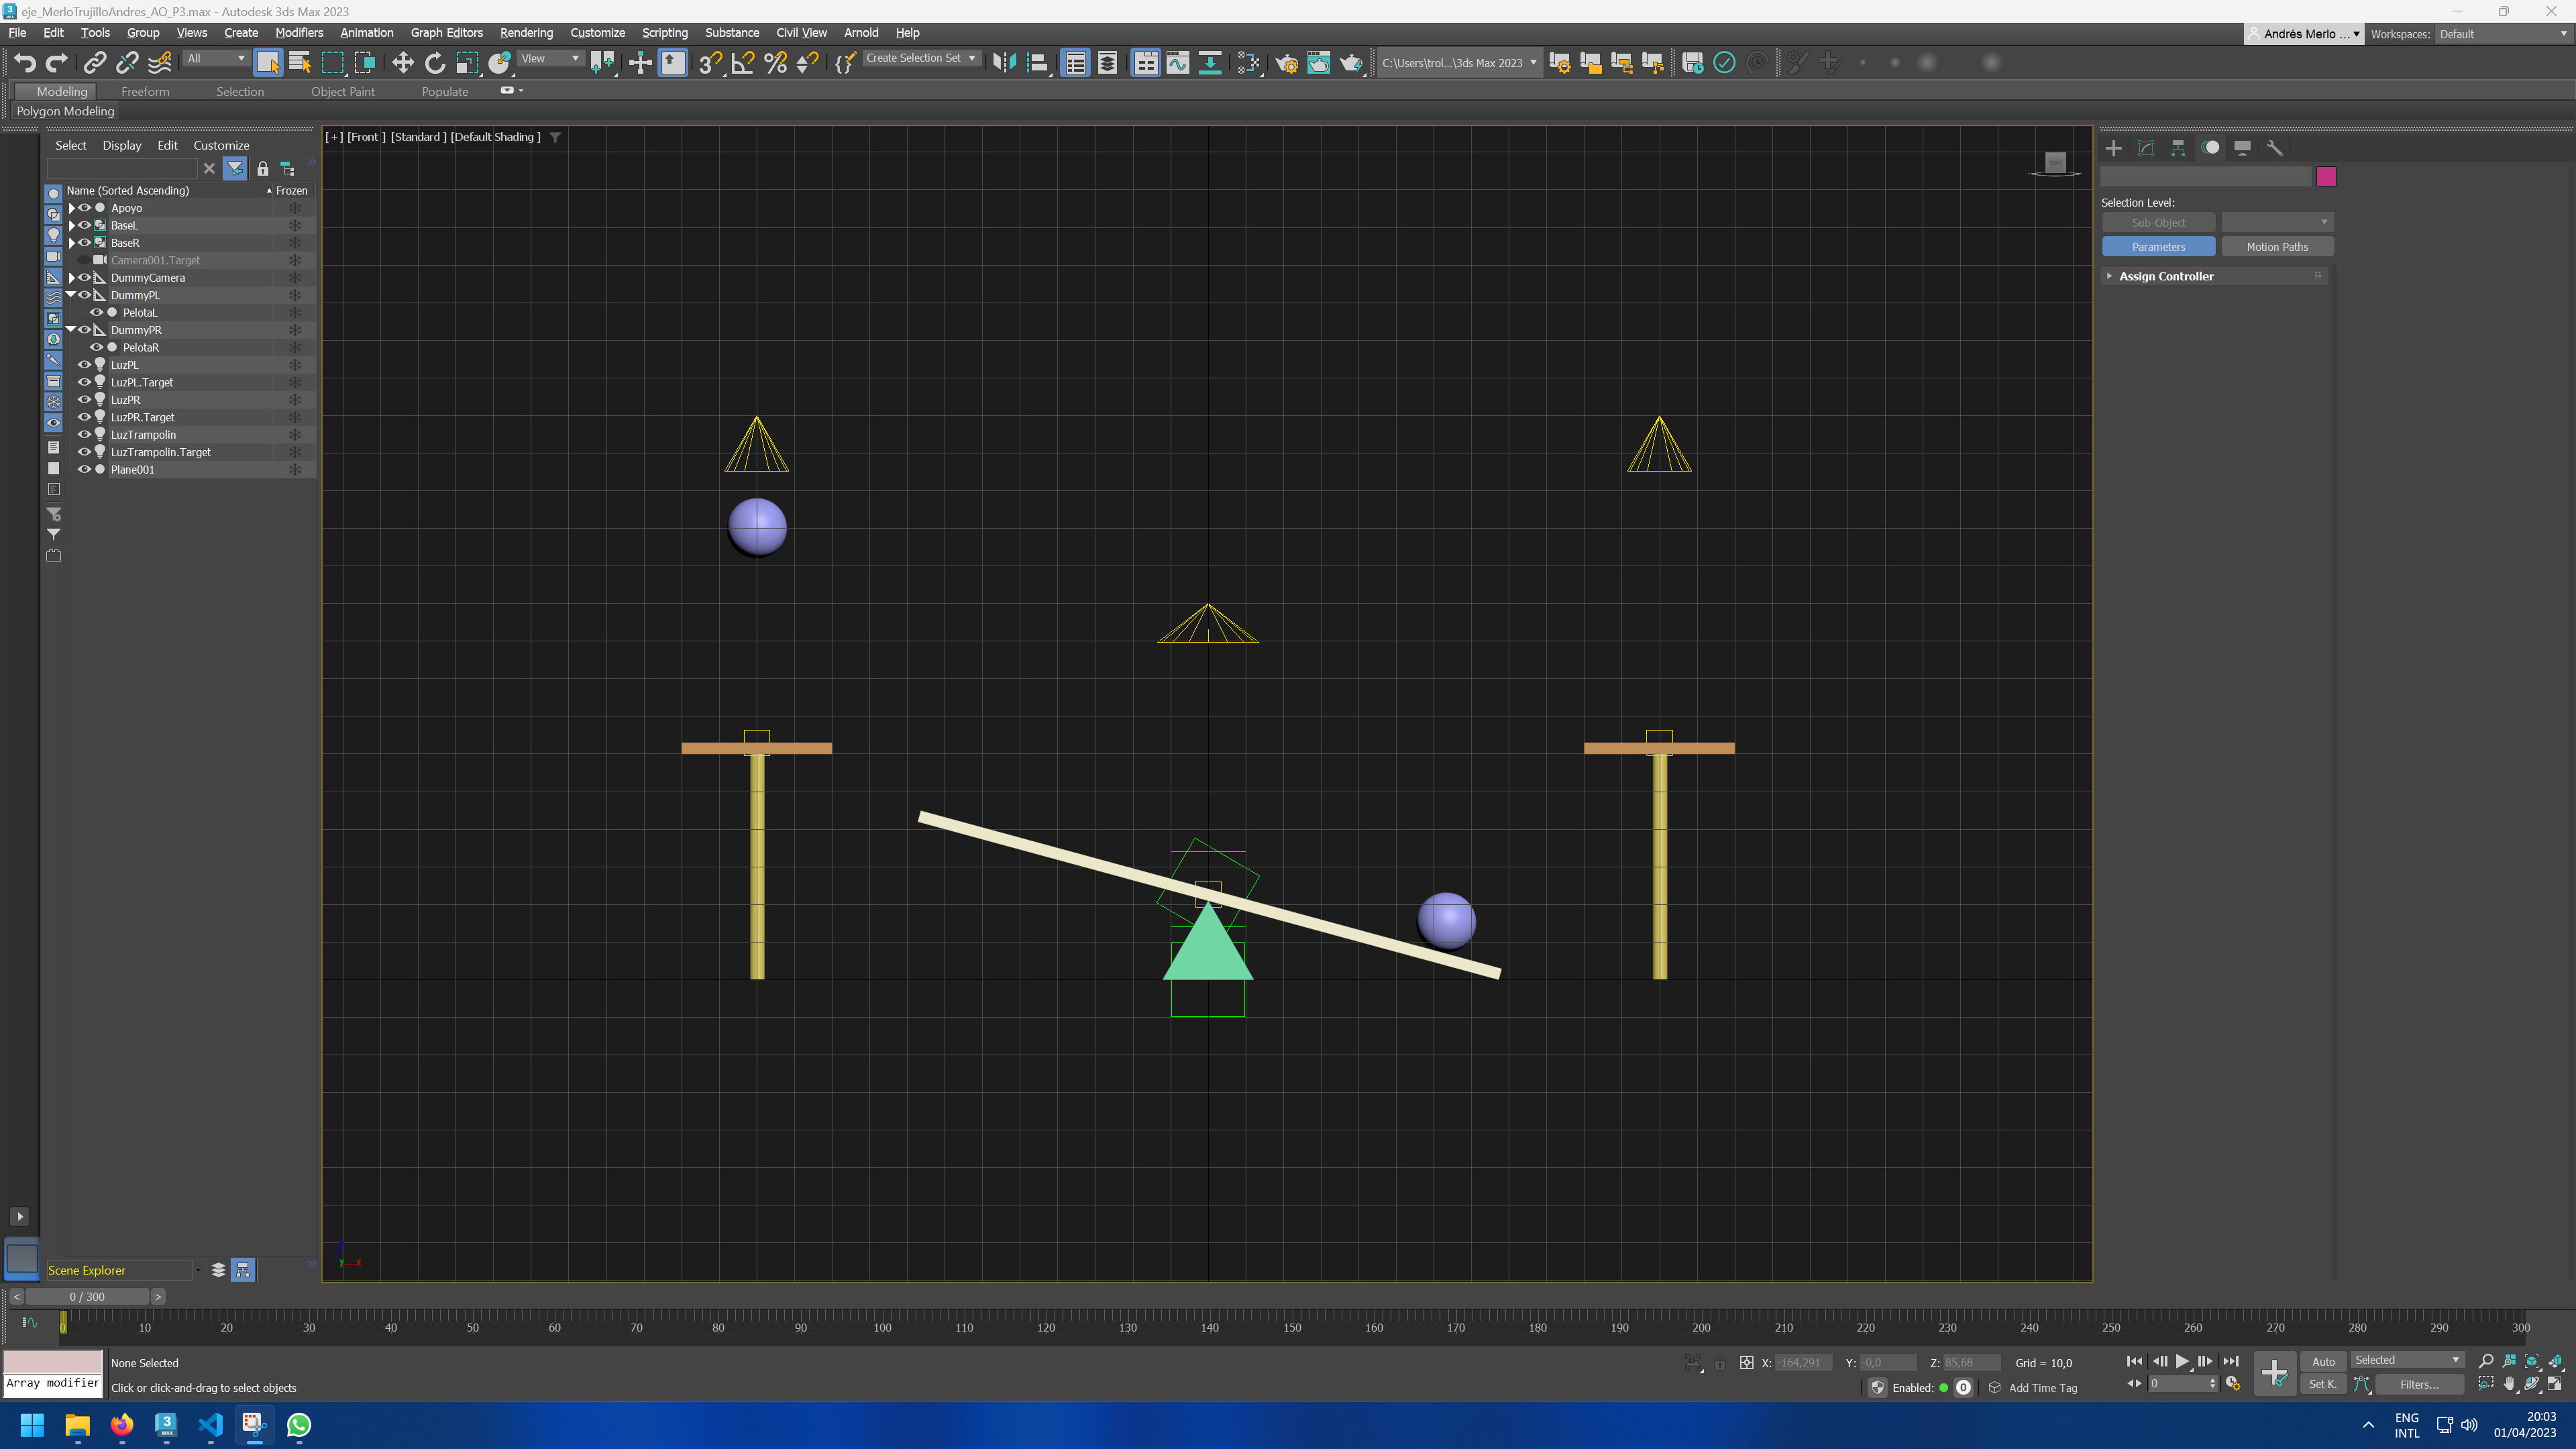
\includegraphics[width=\textwidth]{imagenes/Ejercicio 1/keyframes/0.png}
%         \caption{Pelotas en el instante 0.}
%     \end{subfigure}
%     \hfill
%     %\par\bigskip %si se desea dejar un margen entre la imagen de arriba y de abajo
% 	\begin{subfigure}[t]{0.48\textwidth}
% 	    \centering
% 	    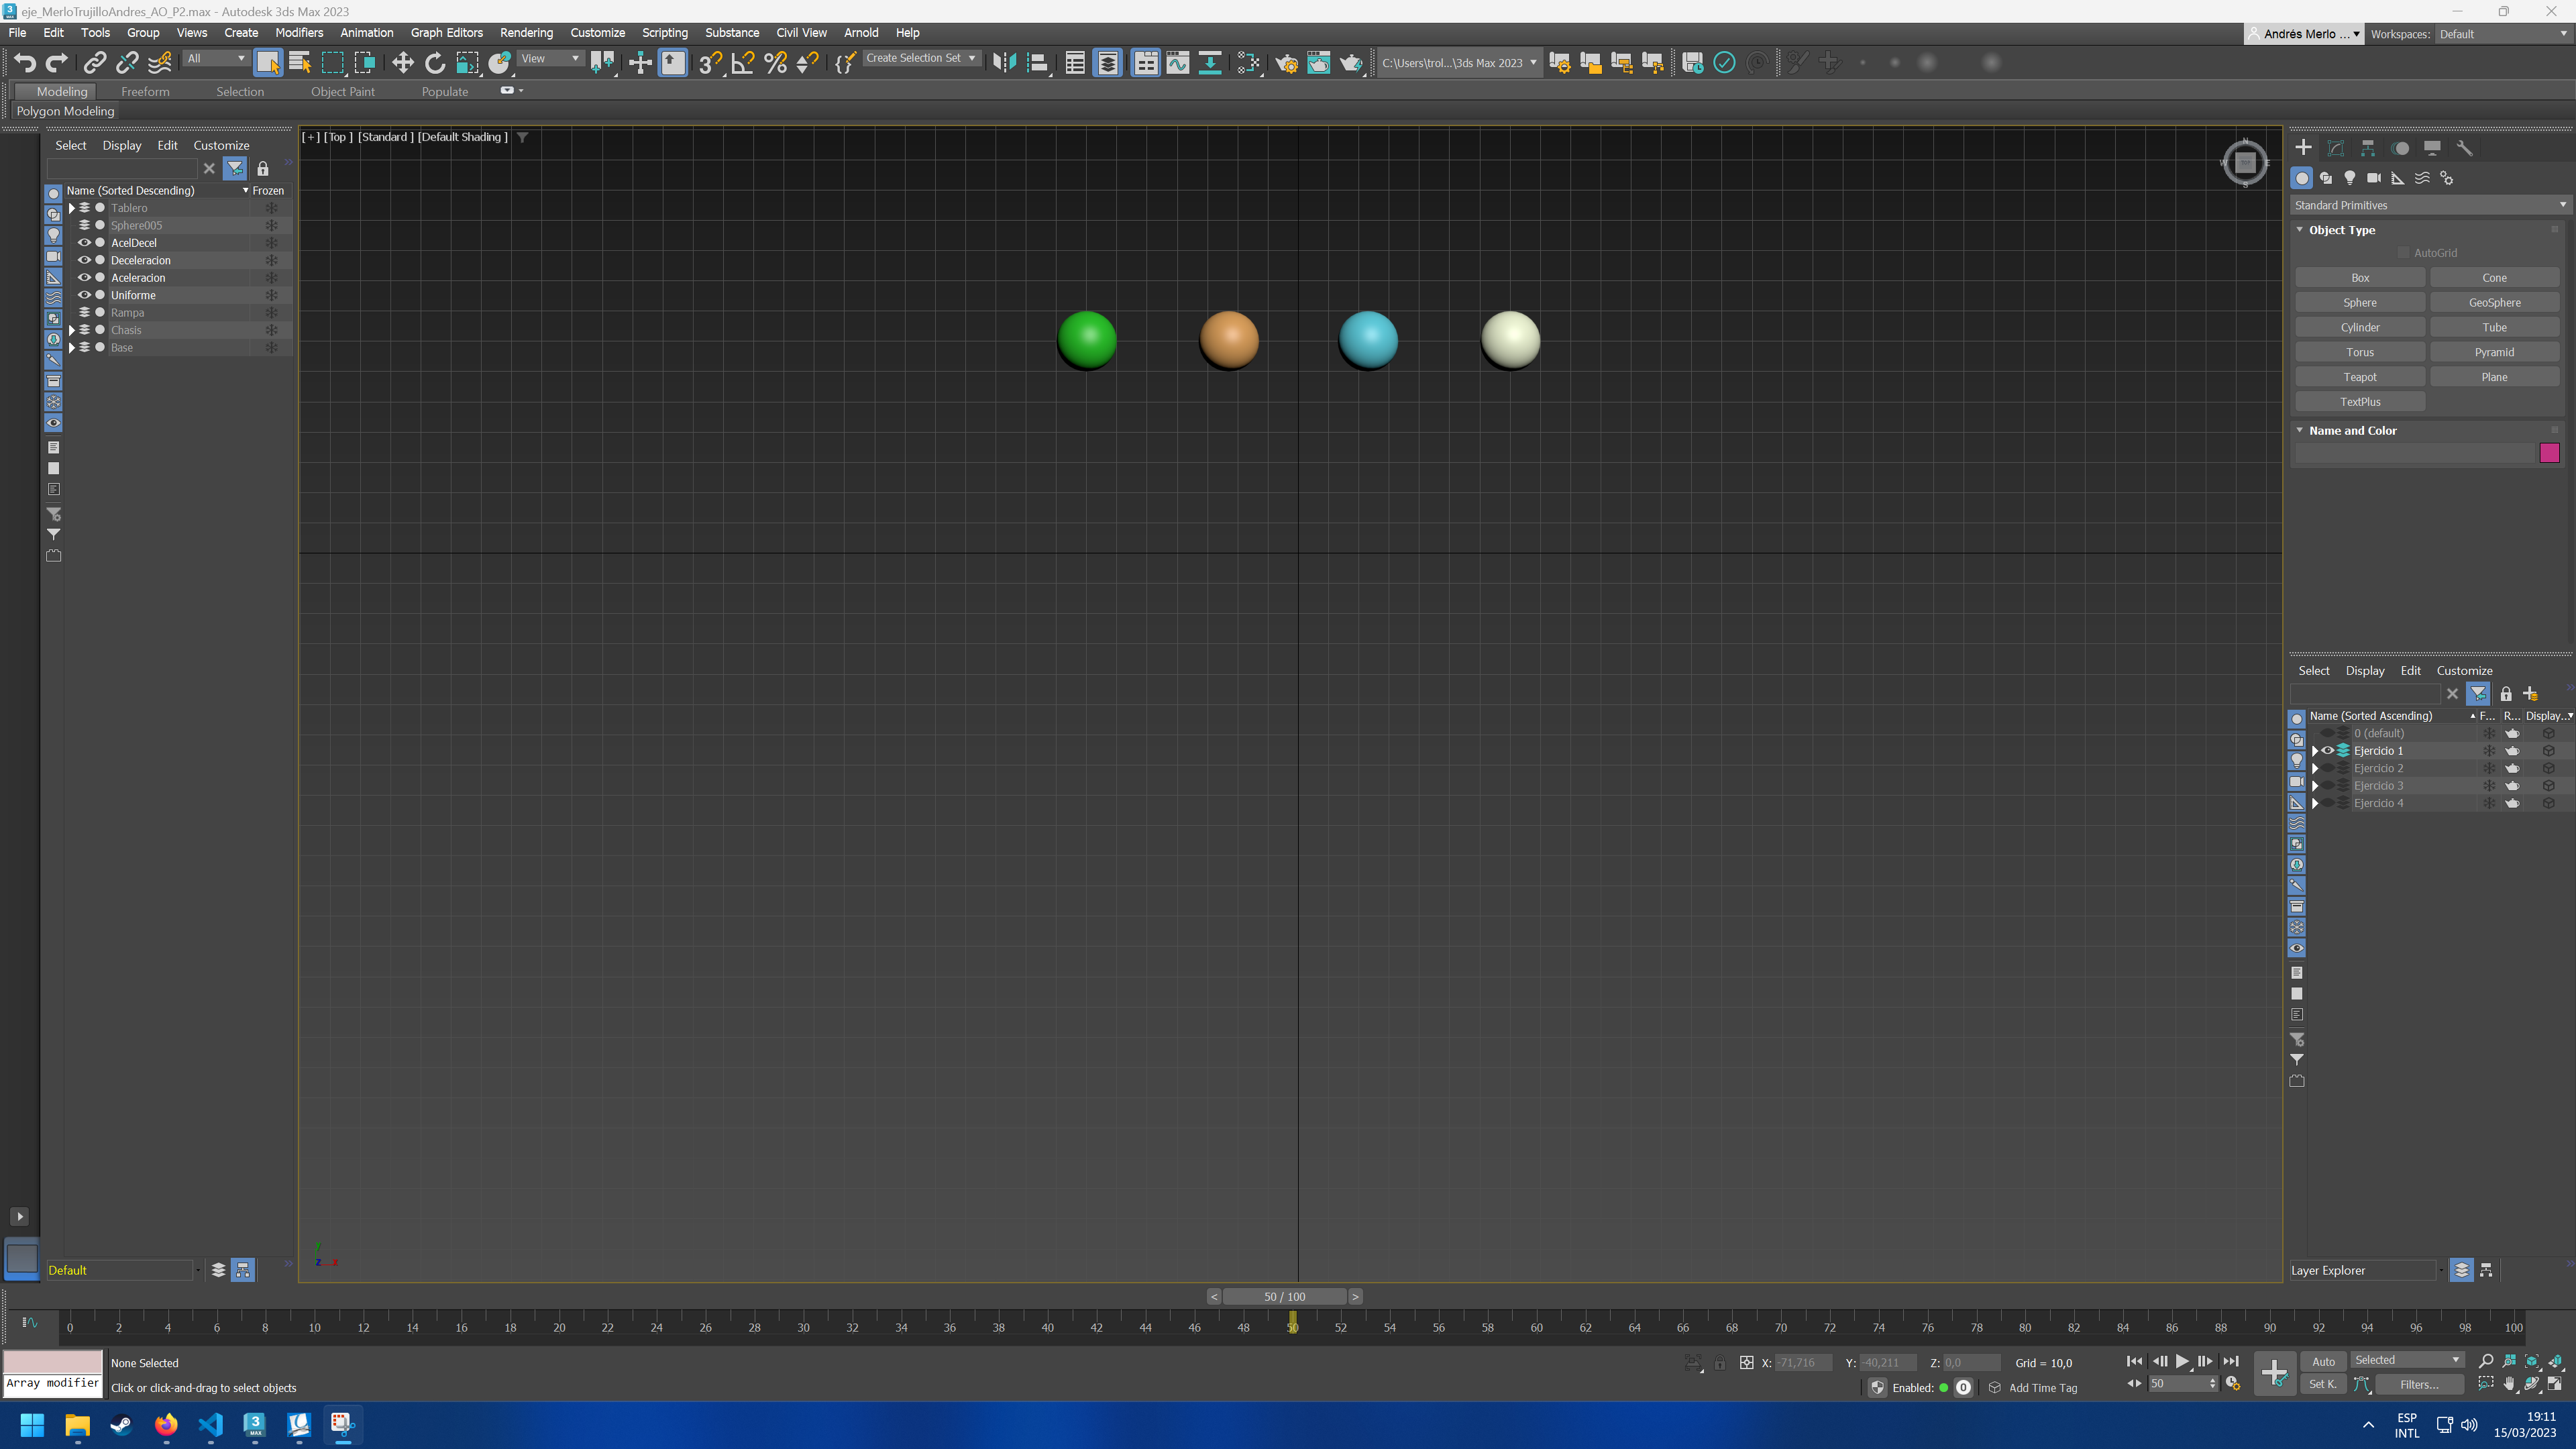
\includegraphics[width=\textwidth]{imagenes/Ejercicio 1/keyframes/50.png}
%         \caption{Pelotas en el instante 50.}
%     \end{subfigure}    
% \end{figure}

% $30 \text{fps} \times 2 \times 5 \text{segundos} = 300 \text{fotogramas} $

\section{Lorem ipsum dolor sit amet, consectetur adipiscing elit. Etiam commodo, nunc a molestie rutrum, lorem justo aliquet quam, suscipit viverra diam sapien eget purus. Aenean ac dapibus lacus, sed fringilla magna. Integer scelerisque arcu id commodo finibus. Etiam posuere arcu id tempor fermentum. Aliquam posuere faucibus eros sed fermentum. Vivamus viverra commodo ipsum vel fermentum. Donec vitae nibh a nibh semper lobortis. Ut eget neque leo. Nulla ullamcorper in nisi nec consectetur. }

...

\end{document}
